\chapter{"superuser" szintű felhasználói felületek, és azok működése}
\label{chap:fejezet7}

A "superuser" szintű felhasználók az oldal adminisztrátorai. Nem tartozik a profiljukhoz sem "Patient" példány, sem "Doctor" példány. A felhasználók személyes adatain kívül mindenhez hozzáférnek az adatbázisban, és mindent joguk van törölni, vagy módosítani. A Django beépített admin felületére is van joguk bejelentkezni. Időpontot foglalni viszont nem tudnak, hasonló okok miatt, mint az orvosok.

\section{Az "Admin" oldal}

Az Admin oldal az "admin.html" fájlban lett megvalósítva, az adminisztrátor ezen az oldalon éri el az összes admin felületet.\\

\begin{figure}[!htbp]
	\caption{Az "Admin" oldal}
	\label{fig:adminpage}
	\centering
	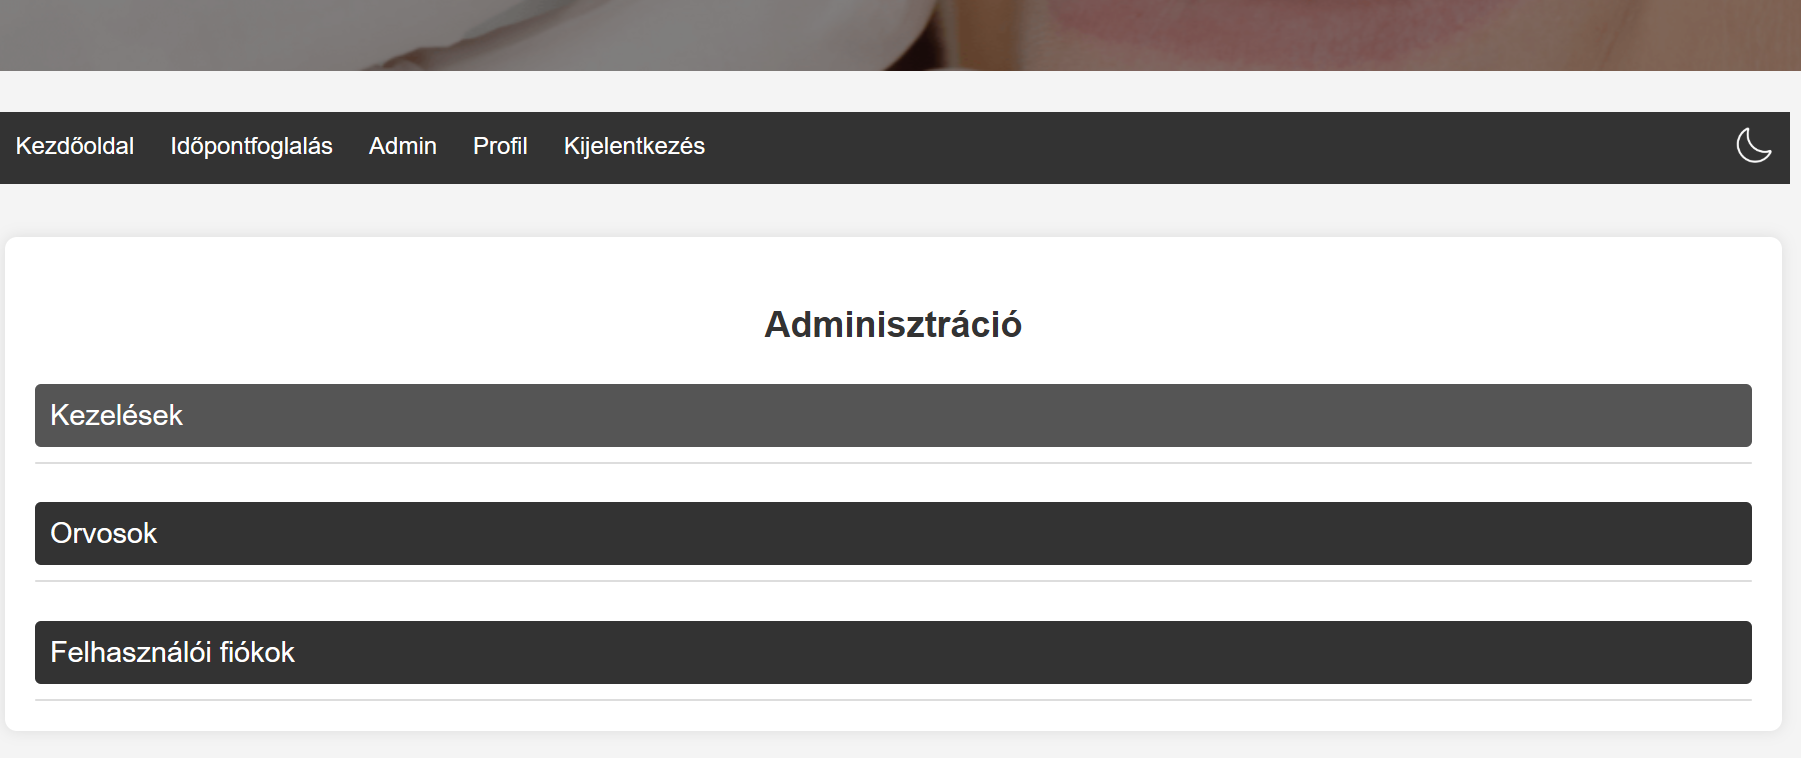
\includegraphics[width=1.0\textwidth]{admin_page.png}
\end{figure}

Az oldalon a 7.1. ábrán látható három lenyíló menü fogadja a felhasználót. Ezekben vannak a kezelések, az orvosok, és a felhasználói fiókok szerkesztési lehetőségei.\\

Ha lenyitja a kezeléseket akkor kilistázza az oldal az adatbázisban található összes megadott kezelést. A lenyíló gomb alatt található egy "Új kezelés hozzáadása" gomb, ami az "add\_treatment.html" oldalra navigálja a felhasználót. Ezen az oldalon a "TreatmentForm" található, amiben megadhatja a hozzáadni kívánt kezelés adatait, majd a "Mentés" gombbal elmentheti, vagy a "Mégsem" gombbal visszatérhet az Admin oldalra.\\

A kilistázott kezeléseknél mindegyikhez jut két gomb: "Törlés", vagy "Szerkesztés".\\

A "Törlés" a "Delete\_treatment.html" fájlba navigálja a felhasználót, ahol megkérdezi az oldal, hogy biztosan törölni kívánja-e a kezelést, és megjeleníti a kezelés adatait is. Az oldalon található "Törlés" gomb értelem szerűen törli, míg a "Mégsem" gomb visszanavigál az Admin oldalra.\\

A "Szerkesztés" gomb az "edit\_treatment.html" oldalra navigál, ahol szintén megjelenik a "TreatmentForm" a kiválasztott kezelés adataival kitöltve. Bármilyen adatot átírhat itt is a felhasználó, az oldalon lévő "Mentés" és "Mégsem" gombok pedig a megszokott módon működnek.\\

Az orvosok lenyíló menüben is hasonló lehetőségek találhatók, kilistázza az oldal az összes adatbázisban szereplő orvost egymás alá, és lehet újat elmenteni, szerkeszteni, és törölni az adatbázisból. Az új hozzáadása és a szerkesztés a "ProfileForm", és "DoctorForm" egítségével történik. Ezekhez a műveletekhez is külön oldalakat készítettem az alábbi fájlokban:

\begin{itemize}
	\item "add\_doctor.html"
	\item "edit\_doctor.html"
	\item "delete\_doctor.html"
\end{itemize}

Fontos, hogy itt az új orvos hozzáadása nem csak egy új "Doctor" példányt ad hozzá az adatbázishoz, hanem először létrehoz egy "RendeloUser"-t is, és annak az $id$-jával hozza létre a "Doctor"-t, hogy az orvos azonnal használhassa a felhasználói fiókját is. Az új orvos létrehozása esetén az orvos a megadott email címére meg is kap egy emailt, amiben megkapja a belépési adatait, hogy meg tudja őket változtatni.\\

A felhasználói fiókok lenyíló menüben ismét az adatbázisban található összes adat fogadja a felhasználót kilistázva, viszont ezeket lehetősége van szűrni a megszokott módon felhasználónév alapján.

\begin{figure}[!htbp]
	\caption{Felhasználói fiókok}
	\label{fig:felhasznaloifiokok}
	\centering
	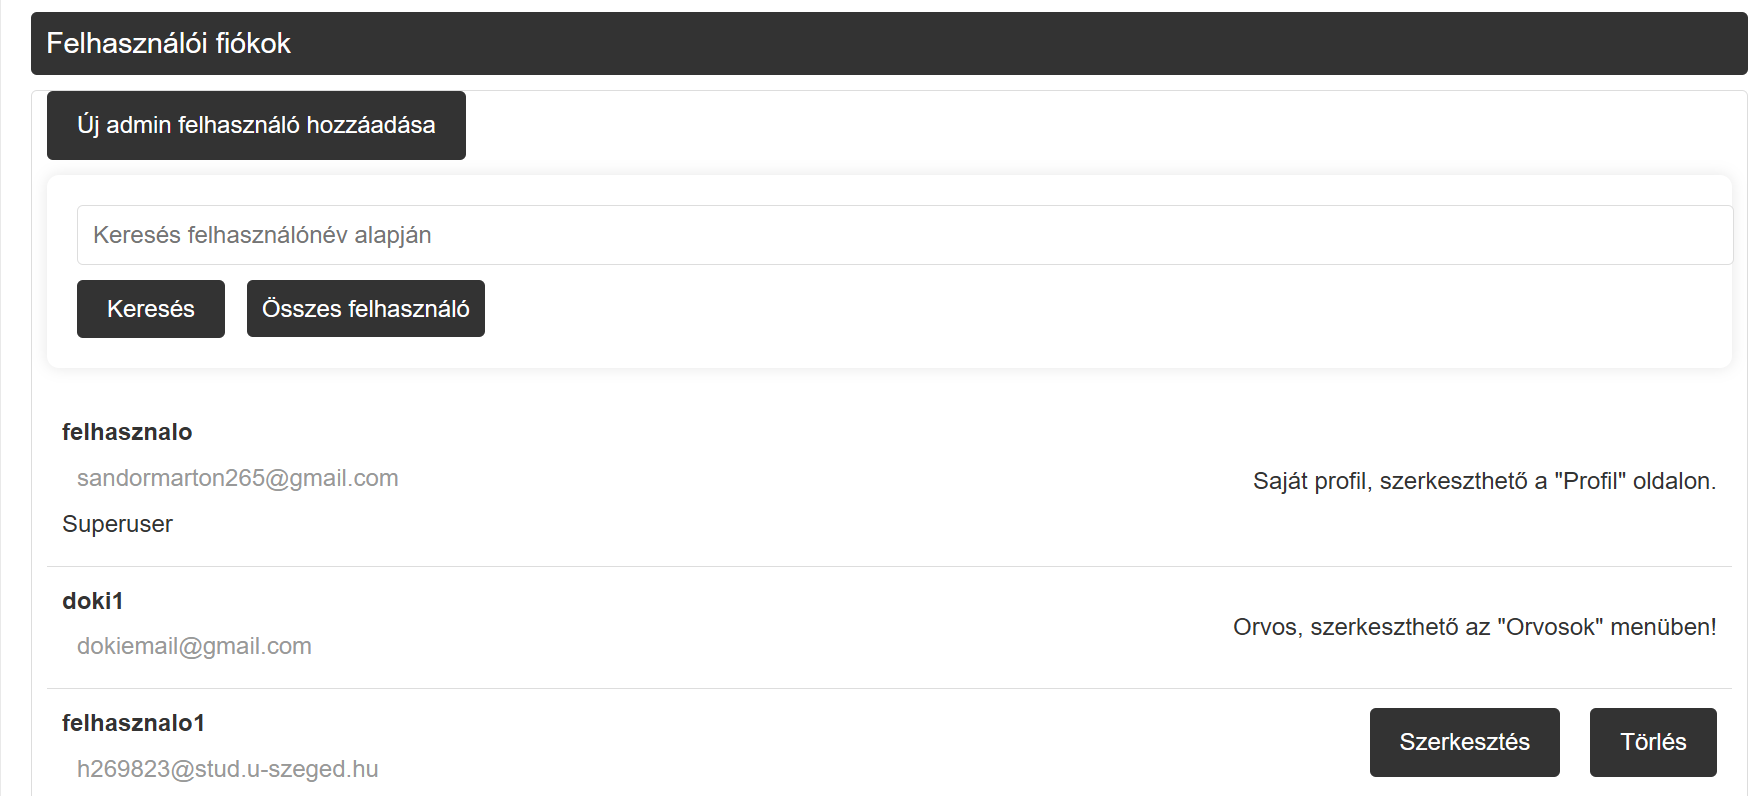
\includegraphics[width=1.0\textwidth]{admin_page_felhasznaloi_fiokok.png}
\end{figure}

Az adminisztrátornak joga van új admin felhasználót hozzáadnia az adatbázishoz, amit az "Új admin felhasználó hozzáadása" gombbal tehet meg. Ez elvezeti az "add\_admin\_user.html" oldalra, amin a "CustomUserCreationForm" segítségével a megszokott módon létrehozhat új rekordot az adatbázisba.\\

A kilistázott felhasználók közül itt nem szerkeszthetők az orvosok, mivel azokhoz ott van az orvosok szerkesztési oldala, és itt nem szerkeszthető, vagy törölhető az admin saját fiókja sem. Ez egy védelem, hogy az alkalmazás ne maradhasson adminisztrátor nélkül. A szerkesztést viszont meg tudja oldani a saját "Profil" oldalán, ami ugyan úgy működik, mint a többi szintű felhasználó esetében.

A "user" szintű felhasználókat, és a többi adminisztrátort pedig ugyan úgy tudja szerkeszteni a "ProfileForm", és a "PatientForm" segítségével, vagy törölni a megszokott módon. Ezekhez is készítettem két külön oldalt:

\begin{itemize}
	\item "edit\_user.html"
	\item "delete\_user.html"
\end{itemize}
